\documentclass[french,10pt]{article}
\input preambule_2013

\begin{document}

%---- On définit ci-dessous les différents styles en fonction du niveau dans l'arbre de proba :
\tikzstyle{level 1}=[level distance=2cm,sibling distance=-3cm]
\tikzstyle{level 2}=[level distance=2.5cm,sibling distance=-1.5cm]

%---- sibling distance négative => les noeuds sont compilés de haut en bas

\begin{tikzpicture}
[grow=right] % dessine l'arbre de gauche à droite. Les options left, up et down sont également disponibles.
    \node{}
%----------------------------------------------------------------------------------------------------------------------
%----------------------------------------------------------------------------------------------------------------------
        child {node {\textcolor{red}{R}}
%----------------------------------------------------------------------------------------------------------------------
                child {node (R1) {\textcolor{red}{R}} % le nom du noeud entre parenthèses permet de réutiliser ce noeud ultérieurement (cf tout en bas)
                         node[right=0.5cm] {$\dfrac{3}{8}\times\dfrac{2}{7} = \dfrac{6}{56}$}
                         node[above=0.75cm,right=0.5cm] {Probabilités :}
                         edge from parent node[above] {\tiny$\dfrac{2}{7}$}
                        }
%----------------------------------------------------------------------------------------------------------------------
                child {node {\textcolor{blue}{B}}
                         node[right=0.5cm] {$\dfrac{3}{8}\times\dfrac{5}{7} = \dfrac{15}{56}$}
                         edge from parent node[below] {\tiny$\dfrac{5}{7}$}
                        }
%----------------------------------------------------------------------------------------------------------------------
           edge from parent node[above] {\tiny$\dfrac{3}{8}$}
        }
%----------------------------------------------------------------------------------------------------------------------
%----------------------------------------------------------------------------------------------------------------------
        child {node {\textcolor{blue}{B}}
%----------------------------------------------------------------------------------------------------------------------
                child {node {\textcolor{red}{R}}
                         node[right=0.5cm] {$\dfrac{5}{8}\times\dfrac{3}{7} = \dfrac{15}{56}$}
                         edge from parent node[above] {\tiny$\dfrac{3}{7}$}
                        }
%----------------------------------------------------------------------------------------------------------------------
                child {node {\textcolor{blue}{B}}
                         node[right=0.5cm] {$\dfrac{5}{8}\times\dfrac{4}{7} = \dfrac{20}{56}$}
                         edge from parent node[below] {\tiny$\dfrac{4}{7}$}
                        }
%----------------------------------------------------------------------------------------------------------------------
            edge from parent node[below] {\tiny$\dfrac{5}{8}$}
        }
;
% Utilisation d'un noeud déjà défini
\draw (R1) node[right=2.5cm] {$\rightarrow\ (R \pv R)$ : issue gagnante};
\end{tikzpicture}






\begin{tikzpicture}
[grow=right] % dessine l'arbre de gauche à droite. Les options left, up et down sont également disponibles.
    \node{}
%----------------------------------------------------------------------------------------------------------------------
%----------------------------------------------------------------------------------------------------------------------
        child {node {R}
%----------------------------------------------------------------------------------------------------------------------
      child {node (R1) {...} % le nom du noeud entre parenthèses permet de réutiliser ce noeud ultérieurement (cf tout en bas)
                         node[right=0.5cm] {...}
                         node[above=0.75cm,right=0.5cm] {}
                         edge from parent node[above] {...}
                        }         
%----------------------------------------------------------------------------------------------------------------------
               child {node {...}
                         node[right=0.5cm] {...}
                         edge from parent node[below] {...}
                        } 
%----------------------------------------------------------------------------------------------------------------------
           edge from parent node[above] {...}
        }
%----------------------------------------------------------------------------------------------------------------------
%----------------------------------------------------------------------------------------------------------------------
        child {node {$\overline{R}$}
%----------------------------------------------------------------------------------------------------------------------
%                child {node {R}
%                         node[right=0.5cm] {$\dfrac{5}{8}\times\dfrac{3}{7} = \dfrac{15}{56}$}
%                         edge from parent node[above] {\tiny$\dfrac{3}{7}$}
%                        }
%%----------------------------------------------------------------------------------------------------------------------
%                child {node {\textcolor{blue}{B}}
%                         node[right=0.5cm] {$\dfrac{5}{8}\times\dfrac{4}{7} = \dfrac{20}{56}$}
%                         edge from parent node[below] {\tiny$\dfrac{4}{7}$}
%                        }
%----------------------------------------------------------------------------------------------------------------------
            edge from parent node[below] {...}
        }
;
% Utilisation d'un noeud déjà défini

\end{tikzpicture}
\end{document} 